\documentclass[tikz,margin=2mm]{standalone}
\pagestyle{empty}

\usepackage{amsmath}
\usepackage{bm}
\usetikzlibrary{positioning,calc,arrows}

% variable styles
\tikzstyle{error} = [ draw=black,fill=gray!50!white,circle, inner sep = 1pt, minimum size = 0.35cm ]
\tikzstyle{latent} = [ draw, circle, inner sep = 1pt, minimum size = 0.45cm ]
\tikzstyle{observed} = [ draw, rectangle, inner sep = 2pt, minimum size = 0.65cm ]
\tikzstyle{measure} = [ draw, rectangle, inner sep = 1pt, minimum size = 0.45cm, outer sep = 0.5pt]
\tikzstyle{refpoint} = [inner sep = 0pt, outer sep = 0pt]


\tikzstyle{edge} = [->]
\tikzstyle{highlightEdge} = [->, very thick]
\tikzstyle{highlightEdge2} = [->, dashed]
\tikzstyle{transform} = [->, very thick, >=triangle 45]

\begin{document}

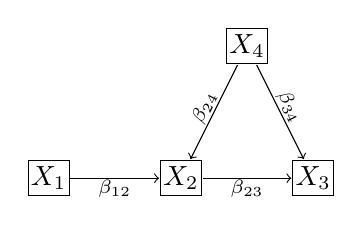
\begin{tikzpicture}[scale=1.2]
	\node[measure] (x1) at ( 0, 0 ) { $ X_1 $ };
	\node[measure] (x2) at ( 1.4, 0 ) { $ X_2 $ };
	\node[measure] (x3) at ( 2.8, 0 ) { $ X_3 $ };
	\node[measure] (x4) at ( 2.1, 1.4 ) { $ X_4 $ };

	\draw[edge](x1) -- (x2) node[midway, below, yshift=0.1cm]{\scriptsize $\beta_{12}$};
	\draw[edge](x2) -- (x3) node[midway, below, yshift=0.1cm]{\scriptsize $\beta_{23}$};
	\draw[edge](x4) -- (x2) node[midway, above, sloped, yshift=-0.1cm]{\scriptsize $\beta_{24}$};
	\draw[edge](x4) -- (x3) node[midway, above, sloped, yshift=-0.1cm]{\scriptsize $\beta_{34}$};
\end{tikzpicture}

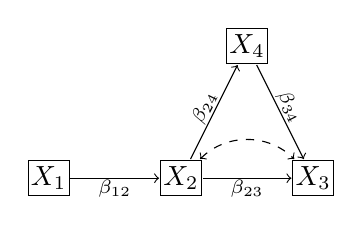
\begin{tikzpicture}[scale=1.2]
	\node[measure] (x1) at ( 0, 0 ) { $ X_1 $ };
	\node[measure] (x2) at ( 1.4, 0 ) { $ X_2 $ };
	\node[measure] (x3) at ( 2.8, 0 ) { $ X_3 $ };
	\node[measure] (x4) at ( 2.1, 1.4 ) { $ X_4 $ };

	\draw[edge](x1) -- (x2) node[midway, below, yshift=0.1cm]{\scriptsize $\beta_{12}$};
	\draw[edge](x2) -- (x3) node[midway, below, yshift=0.1cm]{\scriptsize $\beta_{23}$};
	\draw[edge](x2) -- (x4) node[midway, above, sloped, yshift=-0.1cm]{\scriptsize $\beta_{24}$};
	\draw[edge](x4) -- (x3) node[midway, above, sloped, yshift=-0.1cm]{\scriptsize $\beta_{34}$};
	\draw[<->, dashed](x2) to[bend left=45] (x3);
\end{tikzpicture}

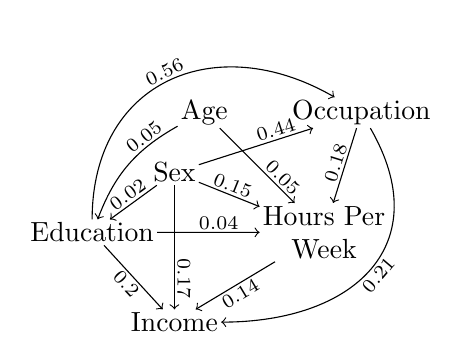
\begin{tikzpicture}[scale=0.95]
\tikzstyle{every node}=[align=center, inner sep=1pt]
	\node (sex) at (-0.7, -0.8) {Sex};
	\node (age) at (-0.3, 0) {Age};
	\node (ed) at (-1.8, -1.6) {Education};
	\node (occ) at (1.8, 0) {Occupation};
	\node (hrpw) at (1.3, -1.6) {Hours Per \\ Week};
	\node (income) at (-0.7, -2.8) {Income};

	\draw[edge]  (age) to[bend right=20] node[above, near start, sloped]{\scriptsize $ 0.05 $} (ed);
	\draw[edge]  (sex) to node[above, sloped] {\scriptsize $ 0.02 $} (ed);
	\draw[edge]  (age) to node[above, near end, sloped] {\scriptsize $ 0.05 $} (hrpw);
	\draw[edge]  (ed) to node[above, pos=0.6, sloped] {\scriptsize $ 0.04 $} (hrpw);
	\draw[edge]  (occ) to node[above, sloped] {\scriptsize $ 0.18 $} (hrpw);
	\draw[edge]  (sex) to node[above, sloped] {\scriptsize $ 0.15 $} (hrpw);
	\draw[edge]  (ed) to node[below, sloped] {\scriptsize $ 0.2 $} (income);
	\draw[edge]  (hrpw) to node[below, sloped] {\scriptsize $ 0.14 $} (income);
	\draw[edge]  (occ) to[out=300, in=0, looseness=1.4] node[below, sloped] {\scriptsize $ 0.21 $} (income.east);
	\draw[edge]  (sex) to node[above, near end, sloped] {\scriptsize $ 0.17 $} (income);
	\draw[edge]  (ed) to[out=90, in=150, looseness=1.3] node[above, sloped] {\scriptsize $ 0.56 $} (occ);
	\draw[edge]  (sex) to node[above, pos=0.7, sloped] {\scriptsize $ 0.44 $} (occ);	
\end{tikzpicture}

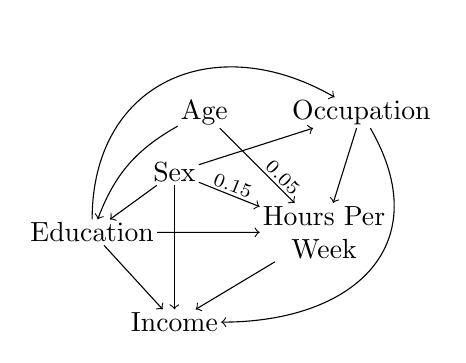
\begin{tikzpicture}[scale=0.95]
\tikzstyle{every node}=[align=center, inner sep=1pt]
	\node (sex) at (-0.7, -0.8) {Sex};
	\node (age) at (-0.3, 0) {Age};
	\node (ed) at (-1.8, -1.6) {Education};
	\node (occ) at (1.8, 0) {Occupation};
	\node (hrpw) at (1.3, -1.6) {Hours Per \\ Week};
	\node (income) at (-0.7, -2.8) {Income};

	\draw[edge]  (age) to [bend right=20] (ed);
	\draw[edge]  (sex) to (ed);
	\draw[edge]  (age) to node[above, near end, sloped] {\scriptsize $ 0.05 $} (hrpw);
	\draw[edge]  (ed) to (hrpw);
	\draw[edge]  (occ) to (hrpw);
	\draw[edge]  (sex) to node[above, sloped] {\scriptsize $ 0.15 $} (hrpw);
	\draw[edge]  (ed) to (income);
	\draw[edge]  (hrpw) to (income);
	\draw[edge]  (occ) to[out=300, in=0, looseness=1.4] (income.east);
	\draw[edge]  (sex) to (income);
	\draw[edge]  (ed) to[out=90, in=150, looseness=1.3] (occ);
	\draw[edge]  (sex) to (occ);	
\end{tikzpicture}

\end{document}
